% flashcards-title: Powers-of-ten scale
% flashcards-desc: A horizontal axis has equally spaced ticks from ten to the minus six through ten to the zero. Circular point A is at ten to the minus five; square point B is at ten to the minus two.
\documentclass[border=6pt]{standalone}
\def\pgfsysdriver{pgfsys-dvisvgm.def}
\usepackage{tikz}
\usetikzlibrary{arrows.meta,positioning,shapes.geometric}
\definecolor{mechInk}{HTML}{172033}
\definecolor{mechBlue}{HTML}{155EEF}
\definecolor{mechOrange}{HTML}{B54708}
\definecolor{mechPale}{HTML}{E8F0FF}
\definecolor{mechGray}{HTML}{667085}
\definecolor{mechLight}{HTML}{D0D5DD}
\tikzset{
  every picture/.style={font=\sffamily\large, text=mechInk},
  mech box/.style={draw=mechInk, line width=1.2pt, rounded corners=4pt,
    fill=white, align=center, minimum height=14mm, inner xsep=5mm},
  mech primary/.style={draw=mechBlue, line width=2.2pt},
  mech secondary/.style={draw=mechOrange, line width=2.2pt, dashed},
  mech guide/.style={draw=mechGray, line width=0.9pt, dashed},
  mech arrow/.style={-{Stealth[length=3.2mm,width=2.4mm]},
    draw=mechInk, line width=1.4pt, line cap=butt},
  mech axis/.style={draw=mechInk, line width=1.2pt},
  mech tick/.style={draw=mechInk, line width=1pt}
}

\begin{document}
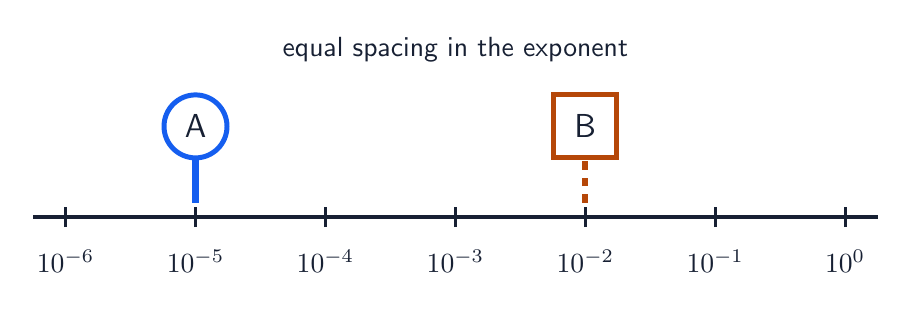
\begin{tikzpicture}[x=1.65cm,y=1cm]
  \draw[mech axis] (-0.25,0) -- (6.25,0);
  \foreach \x/\e in {0/-6,1/-5,2/-4,3/-3,4/-2,5/-1,6/0}{
    \draw[mech tick] (\x,-0.13) -- (\x,0.13);
    \node[below=3mm, font=\sffamily\normalsize] at (\x,0) {$10^{\e}$};
  }
  \draw[mech primary] (1,0.18) -- (1,0.9);
  \node[draw=mechBlue, fill=white, circle, line width=1.8pt,
    minimum size=8mm, inner sep=0pt] at (1,1.15) {A};
  \draw[mech secondary] (4,0.18) -- (4,0.9);
  \node[draw=mechOrange, fill=white, rectangle, line width=1.8pt,
    minimum size=8mm, inner sep=0pt] at (4,1.15) {B};
  \node[above=7mm, font=\sffamily\normalsize] at (3,1.15)
    {equal spacing in the exponent};
\end{tikzpicture}
\end{document}
